\documentclass[a4paper]{article}
\usepackage[utf8]{inputenc}
\usepackage[russian,english]{babel}
\usepackage[T2A]{fontenc}
\usepackage[left=10mm, top=20mm, right=18mm, bottom=15mm, footskip=10mm]{geometry}
\usepackage{indentfirst}
\usepackage{amsmath,amssymb}
\usepackage[italicdiff]{physics}
\usepackage{graphicx}
\usepackage{multirow}
\usepackage{svg}
\graphicspath{{images/}}
\DeclareGraphicsExtensions{.pdf,.png,.jpg}
\usepackage{wrapfig}
\usepackage{caption}
\captionsetup[figure]{name=Рисунок}
\captionsetup[table]{name=Таблица}
\title{\underline{Безынерционные линейные цепи}}
\author{Манро Эйден, Б01-307}
\date{}

\begin{document}
\maketitle
\begin{center}
\Large{\textbf{ }}
\end{center}

\subparagraph{Цель работы:}

\begin{itemize}
    \item Изучение делителей напряжений: получить выходное напряжение 2В при входном 10В;
    \item Изучение параллельных сумматоров и их H-параметров;
    \item Изучение Х-параметров для преобразования "Звезда - Треугольник";
    \item Изучение А-параметров для лестничной структуры.
\end{itemize}

\subparagraph{В работе используются:}

\begin{itemize}
    \item Макетная плата;
    \item Различные резисторы и провода;
    \item Генератор сигналов и осциллограф;
\end{itemize}

\section{Делитель напряжения}

\begin{wrapfigure}{r}{0.4\textwidth}
    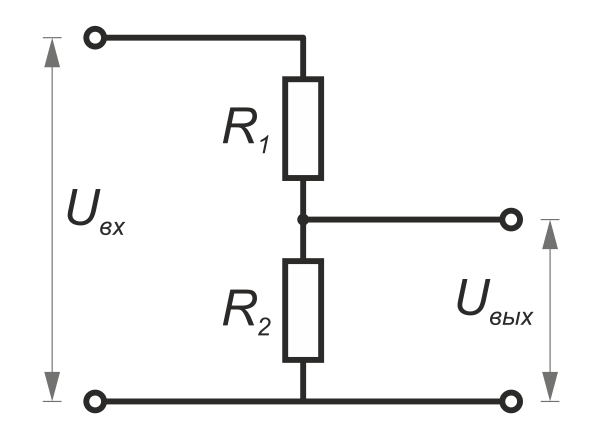
\includegraphics[width = 0.35\textwidth]{splitter.png}
    \caption[width = 0.95\textwidth]{Делитель напряжения}
\end{wrapfigure}

\subsection{Постоянный ток}

Нам нужно получить $E_\text{вых} = 2B$ при входном напряжении $E_\text{вх} = 10B$.

Используя правила Кирхгофа, легко получить:

\begin{equation}
    \frac{E_\text{вх} - E_\text{вых}}{R_1} = \frac{E_\text{вых}}{R_2} \longrightarrow \frac{R_2}{R_1} = \frac{E_\text{вых}}{E_\text{вх} - E_\text{вых}} = \frac{4}{5}
\end{equation}

Выберем $R_2 = 5.6 \ \text{Ом}$, $R_1 = 1.4 \ \text{Ом}$,
тогда при входном напряжении $10B$ мы действительно получаем $2B$ на выходе.
Теперь расчитаем эквивалентную схему, используя пробный резистор.

$U_\text{хх} = (2.04 \pm 0.01)B$

Подключим пробный резистор $R_\text{пр} = (2.92 \pm 0.01)\ \text{Ом}$,
напряжение на концах равно $U = (1.47 \pm 0.01)B$. Тогда из соотношения найдем $R^*$:

\begin{equation}
    \frac{R_\text{пр}}{R^* + R_\text{пр}} = \frac{U}{E} \longrightarrow R^* = R_\text{пр} \frac{E - U}{U} = (1.13 \pm 0.02) \ \text{Ом}
\end{equation}

Значение с хорошей точностью совпало с теоретическим:

\begin{equation}
    R^*_{ref} = \frac{U_{xx}}{I_\text{кз}} = 1.12B
\end{equation}

\subsection{Переменный ток}

Теперь подключим на вход делителя синусоидальное напряжение.
Подключив пробный резистор, оценим коэффициент передачи $K = \frac{u}{e}$.

\begin{equation}
    K = \frac{u}{e} = (0.21 \pm 0.1)
\end{equation}

Значение совпало в пределах погрешности

\section{Параллельный сумматор}

\begin{wrapfigure}[25]{r}{0.35\textwidth}
    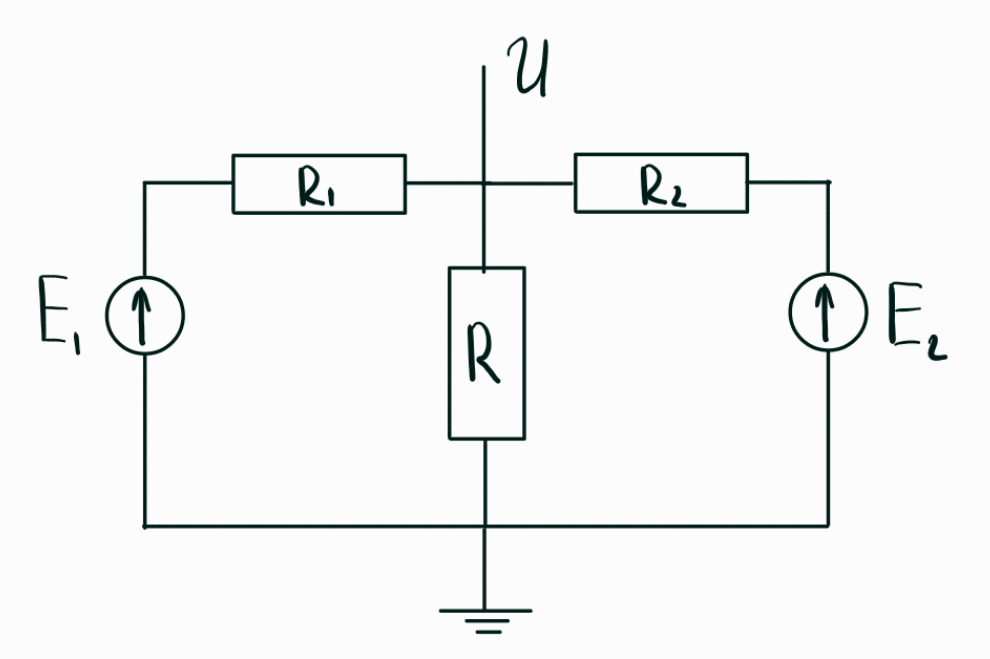
\includegraphics[width = 0.40\textwidth]{summator.png}
    \caption[width = 0.90\textwidth]{Параллельный сумматор}
\end{wrapfigure}

Выход U параллельного сумматора является взвешенной суммой напряжений $E_1$ и $E_2$.

\begin{equation}
    U = \alpha E_1 + \beta E_2
\end{equation}

Приравняем $E_2$ к нулю, тогда легко найти $\alpha$, аналогично и с $\beta$

\begin{equation}
    \alpha = \frac{R || R_2}{R_1 + R || R_2} \qquad
    \beta  = \frac{R || R_1}{R_2 + R || R_1}
\end{equation}

\begin{wrapfigure}[15]{l}{0.4\textwidth}
    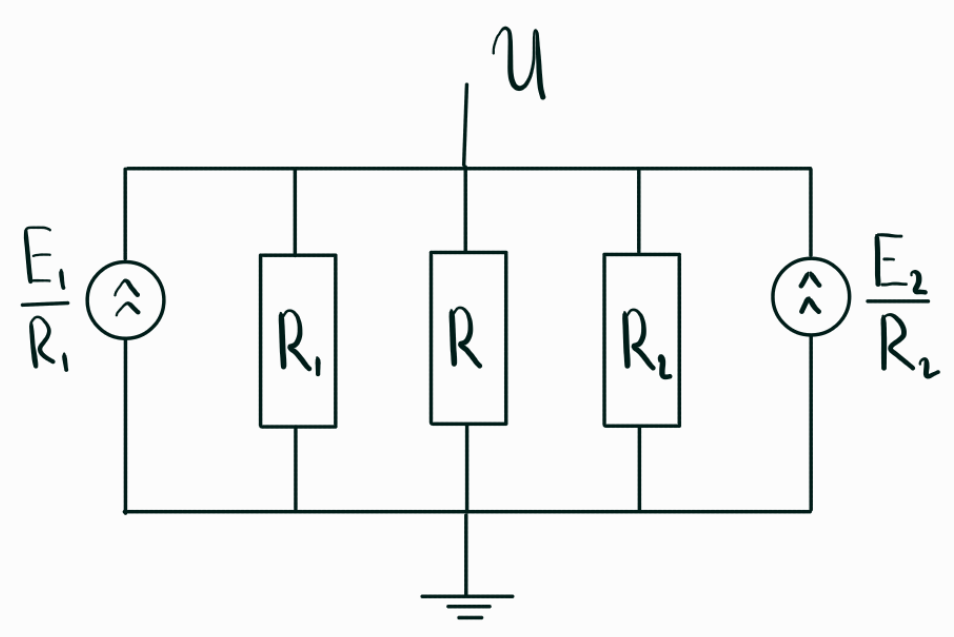
\includegraphics[width = 0.40\textwidth]{summator_eq.png}
    \caption[width = 0.85\textwidth]{Эквивалентная замена сумматора}
\end{wrapfigure}

Заменим $E_1, R_1$ и $E_2, R_2$ эквивалентными схемами с источниками тока.
Теперь очевидно, что:

\begin{equation}
    \frac{\alpha}{\beta} = \frac{R_2}{R_1} \longrightarrow \alpha + \beta = \frac{1}{1 + \frac{R_1 || R_2}{R}}
\end{equation}

Сопротивление эквивалентного источника, соответсвенно,

\begin{equation}
    R^* = R_1 || R || R_2
\end{equation}

Теперь выберем резисторы $R$, $R_1$ и $R_2$ так, чтобы $\alpha = 0.4$, $\beta = 0.2$.

\begin{itemize}
    \item $R_1 = 3.0 \text{кОм}$
    \item $R_2 = 1.5 \text{кОм}$
    \item $R   = 1.5 \text{кОм}$
\end{itemize}

Теперь экспериментально докажем, что $\alpha = 0.4$, $\beta = 0.2$.
Сперва соберем схему на макетной плате, закоротим $E_2$, \newline
$U = (3.98 \pm 1)B$, а значит $\alpha = (0.39 \pm 0.01)$ - совпало в пределах погрешности.
Аналогично, $\beta = (0.19 \pm 0.01)$.

Сравним также внутреннее сопротивление сумматора $R^*$. Аналогично, пробным зарядом получим

\begin{equation}
    R^* = (0.57 \pm 0.02) \ \text{Ом}
\end{equation}

Получилось близко к реальному значению \newline $R_\text{ref} = R_1 || R || R_2 = 0.6 \ \text{Ом}$

\\\

\\\

\\\

\\\

\section{H - параметры}

Проверим формулы для H-параметров T-образной схемы,
аналогичной параллельному сумматору с тремя различными резисторами

\[
\begin{bmatrix}
    U_1\\
    I_2
\end{bmatrix}
 =
\begin{bmatrix}
    h_{11} & h_{12}\\
    h_{21} & h_{22}
\end{bmatrix}
\begin{bmatrix}
    I_1\\
    U_2
\end{bmatrix}
 =
\begin{bmatrix}
    R_1 + R_3||R_2         & \frac{R_3}{R_3 + R_2} \\
    -\frac{R_3}{R_3 + R_2} & \frac{1}{R_3 + R_2}
\end{bmatrix}
\begin{bmatrix}
    I_1\\
    U_2
\end{bmatrix}
\]

Сперва занулим $U_2$, тогда 1) $U_1 = h_{11} * I_1 \longrightarrow h_{11} = R_1 + R_3 || R_2$

\hspace{4.2cm} 2) $I_2 = h_{21} * I_1 \longrightarrow h_{21} = -\frac{R_3}{R_3 + R_2}$

\vspace{0.3cm}

Теперь занулим $I_1$, тогда 1) $U_1 = h_{12} * U_2 \longrightarrow h_{12} = \frac{R_3}{R_3 + R_2}$

\hspace{4.05cm} 2) $I_2 = h_{22} * U_2 \longrightarrow h_{22} = \frac{1}{R_3 + R_2}$

Измерения в Micro-Cap также подтверждают вычисленные значения.

\newpage

\section{Звезда и тругольник}

Для той же схемы определим X-параметры.

\[
\begin{bmatrix}
    U_1\\
    U_2
\end{bmatrix}
 =
\begin{bmatrix}
    X_{11} & X_{12}\\
    X_{21} & X_{22}
\end{bmatrix}
\begin{bmatrix}
    I_1\\
    I_2
\end{bmatrix}
 =
\begin{bmatrix}
    R_1 + R_3 & R_3       \\
    R_3       & R_2 + R_3
\end{bmatrix}
\begin{bmatrix}
    I_1\\
    I_2
\end{bmatrix}
\]

Сперва занулим $I_2$, тогда 1) $U_1 = X_{11} * I_1 \longrightarrow X_{11} = R_1 + R_3$

\hspace{4.10cm}             2) $U_2 = X_{21} * I_1 \longrightarrow X_{21} = R_3$
\vspace{0.3cm}

Теперь занулим $I_1$, тогда 1) $U_1 = X_{12} * I_2 \longrightarrow X_{12} = R_3$

\hspace{4.05cm}             2) $U_2 = X_{22} * I_2 \longrightarrow X_{22} = R_2 + R_3$
\vspace{0.3cm}

Теперь используем преобразование "Звезда - Треугольник".
\\
Измерения в Micro-Cap показывают, что от преобразований значения четырехполюсника не меняются,
также они показывают верность полученных X-параметров

\section{Лестничная структура}

\begin{figure}[h!]
    \centering
    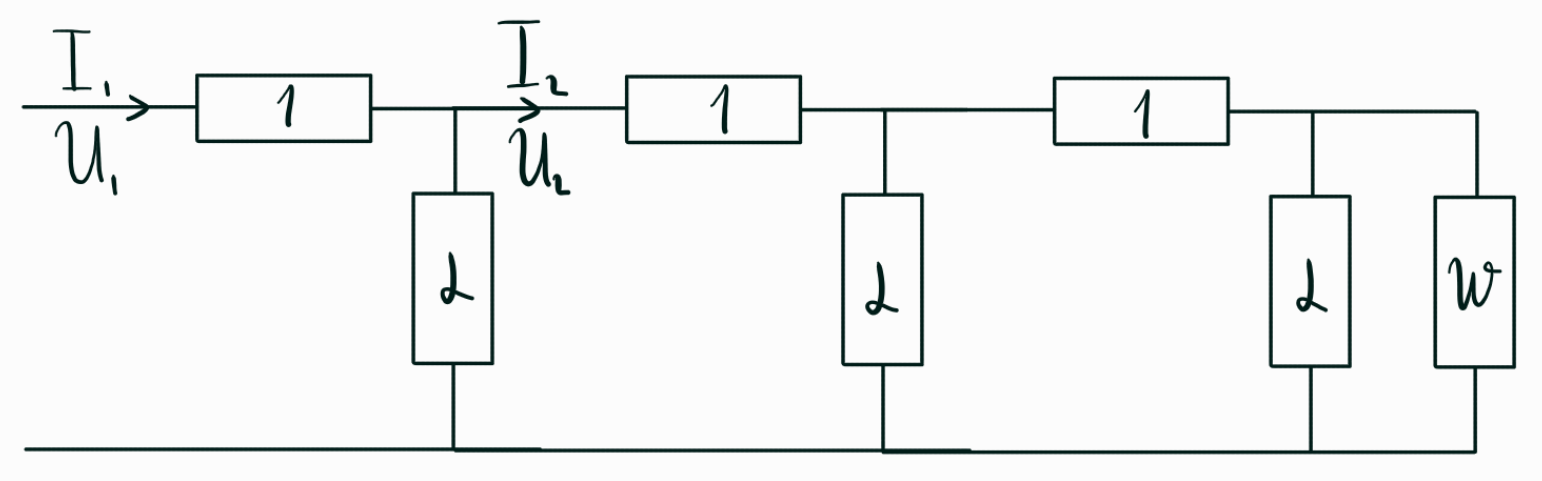
\includegraphics[width=0.5\pdfpagewidth]{stairs.png}
    \caption{Лестничная структура}
\end{figure}

Из условия $w = \frac{U_2}{I_2} = \frac{U_1}{I_1}$ получим:

\begin{equation}
    A_{11} + \frac{A_{12}}{w} = A_{21} w + A_{22} = \gamma \longrightarrow w = \frac{1 + \sqrt{1 + 4\alpha}}{2}
\end{equation}

Исследуя лестничные схемы в Micro-Cap, легко заметить, что напряжение и сила тока в каждом
следующем узле умножается на $\gamma$. Это легко выводится:

\begin{equation}
    U_2 = A_{11} U_1 + A_{12} I_1 = (A_{11} + \frac{A_{12}}{w})U_1 = \gamma U_1
\end{equation}
\begin{equation}
    I_2 = A_{21} U_1 + A_{22} I_1 = (A_{21} + \frac{A_{12}}{w})I_1 = \gamma I_1
\end{equation}

\newpage

\subsection{ЦАП}

Используя данную структуру, можно с легкостью сделать ЦАП.

\begin{figure}[h!]
    \centering
    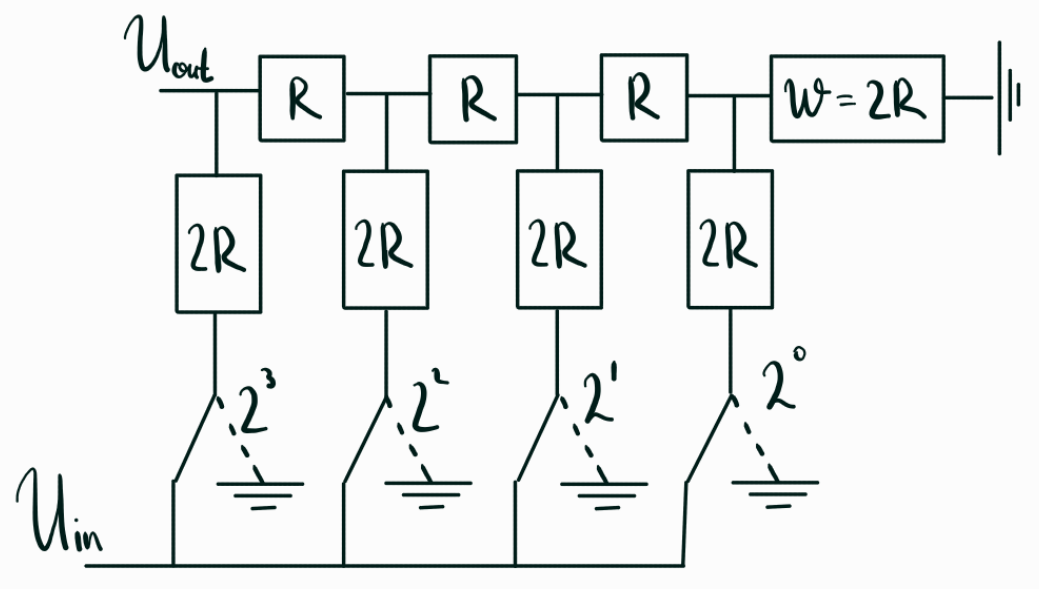
\includegraphics[width=0.5\pdfpagewidth]{dac.png}
    \caption{Лестничная структура}
\end{figure}

Выходное напряжение считается по формуле:
\begin{equation}
    U_\text{out} = U_\text{in} \frac{\text{value}}{2^N},
\end{equation}

где $\text{value}$ - значение, полученное складыванием степеней двойки

$N$ - количество резисторов с номиналом $2R$

\end{document}
